\documentclass[notes,11pt, aspectratio=169]{beamer}

\usepackage{pgfpages}
% These slides also contain speaker notes. You can print just the slides,
% just the notes, or both, depending on the setting below. Comment out the want
% you want.
\setbeameroption{hide notes} % Only slide
%\setbeameroption{show only notes} % Only notes
%\setbeameroption{show notes on second screen=right} % Both

\usepackage{helvet}
\usepackage[default]{lato}
\usepackage{array}
\usepackage{tgbonum}

\usepackage{tikz}
\usepackage{verbatim}
\setbeamertemplate{note page}{\pagecolor{yellow!5}\insertnote}
\usetikzlibrary{positioning}
\usetikzlibrary{snakes}
\usetikzlibrary{calc}
\usetikzlibrary{arrows}
\usetikzlibrary{decorations.markings}
\usetikzlibrary{shapes.misc}
\usetikzlibrary{matrix,shapes,arrows,fit,tikzmark}
\usepackage{amsmath}
\usepackage{mathpazo}
\usepackage{hyperref}
\usepackage{lipsum}
\usepackage{multimedia}
\usepackage{graphicx}
\usepackage{multirow}
\usepackage{graphicx}
\usepackage{dcolumn}
\usepackage{bbm}
\newcolumntype{d}[0]{D{.}{.}{5}}

\usepackage{changepage}
\usepackage{appendixnumberbeamer}
\newcommand{\beginbackup}{
   \newcounter{framenumbervorappendix}
   \setcounter{framenumbervorappendix}{\value{framenumber}}
   \setbeamertemplate{footline}
   {
     \leavevmode%
     \hline
     box{%
       \begin{beamercolorbox}[wd=\paperwidth,ht=2.25ex,dp=1ex,right]{footlinecolor}%
%         \insertframenumber  \hspace*{2ex} 
       \end{beamercolorbox}}%
     \vskip0pt%
   }
 }
\newcommand{\backupend}{
   \addtocounter{framenumbervorappendix}{-\value{framenumber}}
   \addtocounter{framenumber}{\value{framenumbervorappendix}} 
}


\usepackage{graphicx}
\usepackage[space]{grffile}
\usepackage{booktabs}
\newcommand\independent{\protect\mathpalette{\protect\independenT}{\perp}}
\def\independenT#1#2{\mathrel{\rlap{$#1#2$}\mkern2mu{#1#2}}}
\DeclareMathOperator{\Supp}{Supp}

% These are my colors -- there are many like them, but these ones are mine.
\definecolor{blue}{RGB}{0,114,178}
\definecolor{red}{RGB}{213,94,0}
\definecolor{yellow}{RGB}{240,228,66}
\definecolor{green}{RGB}{0,158,115}

\hypersetup{
  colorlinks=false,
  linkbordercolor = {white},
  linkcolor = {blue}
}


%% I use a beige off white for my background
\definecolor{MyBackground}{RGB}{255,253,218}

%% Uncomment this if you want to change the background color to something else
%\setbeamercolor{background canvas}{bg=MyBackground}

%% Change the bg color to adjust your transition slide background color!
\newenvironment{transitionframe}{
  \setbeamercolor{background canvas}{bg=yellow}
  \begin{frame}}{
    \end{frame}
}

\setbeamercolor{frametitle}{fg=blue}
\setbeamercolor{title}{fg=black}
\setbeamertemplate{footline}[frame number]
\setbeamertemplate{navigation symbols}{} 
\setbeamertemplate{itemize items}{-}
\setbeamercolor{itemize item}{fg=blue}
\setbeamercolor{itemize subitem}{fg=blue}
\setbeamercolor{enumerate item}{fg=blue}
\setbeamercolor{enumerate subitem}{fg=blue}
\setbeamercolor{button}{bg=MyBackground,fg=blue,}



% If you like road maps, rather than having clutter at the top, have a roadmap show up at the end of each section 
% (and after your introduction)
% Uncomment this is if you want the roadmap!
% \AtBeginSection[]
% {
%    \begin{frame}
%        \frametitle{Roadmap of Talk}
%        \tableofcontents[currentsection]
%    \end{frame}
% }
\setbeamercolor{section in toc}{fg=blue}
\setbeamercolor{subsection in toc}{fg=red}
\setbeamersize{text margin left=1em,text margin right=1em} 

\newenvironment{wideitemize}{\itemize\addtolength{\itemsep}{10pt}}{\enditemize}

\usepackage{environ}
\NewEnviron{videoframe}[1]{
  \begin{frame}
    \vspace{-8pt}
    \begin{columns}[onlytextwidth, T] % align columns
      \begin{column}{.70\textwidth}
        \begin{minipage}[t][\textheight][t]
          {\dimexpr\textwidth}
          \vspace{8pt}
          \hspace{4pt} {\Large \sc \textcolor{blue}{#1}}
          \vspace{8pt}
          
          \BODY
        \end{minipage}
      \end{column}%
      \hfill%
      \begin{column}{.38\textwidth}
        \colorbox{green!20}{\begin{minipage}[t][1.2\textheight][t]
            {\dimexpr\textwidth}
            Face goes here
          \end{minipage}}
      \end{column}%
    \end{columns}
  \end{frame}
}

\title[]{\textcolor{blue}{Linear Regression I: Inference}}
\author[PGP]{}
\institute[FRBNY]{\small{Paul Goldsmith-Pinkham}}
\date{\today}


\begin{document}

%%% TIKZ STUFF
\tikzset{   
        every picture/.style={remember picture,baseline},
        every node/.style={anchor=base,align=center,outer sep=1.5pt},
        every path/.style={thick},
        }
\newcommand\marktopleft[1]{%
    \tikz[overlay,remember picture] 
        \node (marker-#1-a) at (-.3em,.3em) {};%
}
\newcommand\markbottomright[2]{%
    \tikz[overlay,remember picture] 
        \node (marker-#1-b) at (0em,0em) {};%
}
\tikzstyle{every picture}+=[remember picture] 
\tikzstyle{mybox} =[draw=black, very thick, rectangle, inner sep=10pt, inner ysep=20pt]
\tikzstyle{fancytitle} =[draw=black,fill=red, text=white]
%%%% END TIKZ STUFF

% Title Slide
\begin{frame}
\maketitle

\end{frame}

% INTRO
\begin{frame}{Linear Regression and Inference}
\begin{columns}[T] % align columns
\begin{column}{.8\textwidth}
  \begin{wideitemize}
  \item Today, we'll be focusing on the simple linear model, and studying various cases for understanding inference
    \begin{itemize}
    \item So far we've focused on \emph{identification} -- e.g. what estimands can we know from the data generating process?
    \item Now, given estimators for these estimands, we want to discuss uncertainty and inference
    \end{itemize}
  \item Let's define some notation to start. We'll consider a sample of size $n$:
    \begin{itemize}
    \item causal variable $D_{i}$ (can be continuous valued) $\rightarrow  \; \mathbf{D}_{n}$;
    \item outcome $Y_{i} \rightarrow  \; \mathbf{Y}_{n}$;
%    \item potential outcome will be defined as $Y_{i}^{*}(D_{i})$, where $Y_{i} = Y_{i}^{*}(D_{i})$;
    \item controls $X_{i}$ (relevant for exogeneity, and can be vector valued)  $\rightarrow  \; \mathbf{X}_{n}$.
    \end{itemize}
  \item We'll assume SUTVA holds, and that $D_{i}$ is exogeneous
    conditional on $X_{i}$
  \end{wideitemize}
  \end{column}%
  \hfill%
  \begin{column}{.5\textwidth}
  \end{column}
\end{columns}
\end{frame}

\begin{frame}{Start with the traditional model-based approach}
\begin{columns}[T] % align columns
\begin{column}{.8\textwidth}
  \begin{wideitemize}
  \item Regression is typically written as
    \begin{equation*}
      Y_{i} = X_{i}\gamma + D_{i}\tau + \epsilon_{i},
    \end{equation*}
    where $\epsilon_{i}$ denotes the error term, and is driving the
    randomness to estimate $\tau$ (and $\gamma$). To see this, let
    $W_{i} = (X_{i}, D_{i})$ such that
    \begin{equation*}
      Y_{i} = W_{i}\beta + \epsilon_{i}.
    \end{equation*}
  \item Note that $\hat{\beta} = \beta + (\mathbf{W}_{n}'\mathbf{W}_{n})^{-1}\mathbf{W}_{n}'\boldsymbol{\epsilon}_{n}$
    \begin{itemize}
    \item Typically we take $\mathbf{W}_{n}$ as given, and so the
      uncertainty (in the model based world) is driven by $\epsilon_{i}$
    \end{itemize}
  \end{wideitemize}
  \end{column}%
  \hfill%
  \begin{column}{.5\textwidth}
  \end{column}
\end{columns}
  
\end{frame}

\begin{frame}{Start with the traditional model-based approach}
\begin{columns}[T] % align columns
\begin{column}{.8\textwidth}
  \begin{wideitemize}
  \item The variance of the estimator of $\hat{\beta}$ is
    \begin{equation}
      \mathbb{V}(\hat{\beta} |\mathbf{W}_{n}) = (\mathbf{W}_{n}'\mathbf{W}_{n})^{-1}\mathbf{W}_{n}'\mathbb{E}(\boldsymbol{\epsilon}_{n}\boldsymbol{\epsilon}_{n}'|\mathbf{W}_{n})\mathbf{W}_{n} (\mathbf{W}_{n}'\mathbf{W}_{n})^{-1}
    \end{equation}
    Everything pivots around the structure of
    $\mathbb{E}(\boldsymbol{\epsilon}_{n}\boldsymbol{\epsilon}_{n}'|\mathbf{W}_{n}) = \Omega_{n}$. The simplest case we can consider is homoskedasticity, where $\Omega = \sigma^{2}I_{n}$.
    \item This beautifully simplifies our variance:
    
    \begin{equation}
      \mathbb{V}(\hat{\beta})_{homoskedastic} = \sigma^{2} (\mathbf{W}_{n}'\mathbf{W}_{n})^{-1}
    \end{equation}
  \item What is the content of this assumption? That $Cov(\epsilon_{i},\epsilon_{j}) = 0$ and  $Var(\epsilon_{i} |W_{i}) = Var(\epsilon_{i})$.
  \item Feasible estimator ($k =$ number of regressors):
    \begin{equation}
      \hat{\mathbb{V}}(\hat{\beta})_{homoskedastic} = \hat{\sigma}^{2} (\mathbf{W}_{n}'\mathbf{W}_{n})^{-1}  \qquad \hat{\sigma}^{2} = (n-k-1)^{-1}\boldsymbol{\hat{\epsilon}}_{n}' \boldsymbol{\hat{\epsilon}}_{n} 
    \end{equation}
  \end{wideitemize}
  \end{column}%
  \hfill%
  \begin{column}{.5\textwidth}
  \end{column}
\end{columns}
  
\end{frame}

\begin{frame}{Start with the traditional model-based approach}
\begin{columns}[T] % align columns
\begin{column}{.8\textwidth}
  \begin{wideitemize}
  \item Under heteroskedasticity (which implies that $Var(\epsilon_{i} | W_{i}) = \sigma^{2}(W_{i})$, the robust estimator comes from Eicker (1967), Huber (1967) and White (1980) [EHW]:
    \begin{equation*}
      \hat{\mathbb{V}}(\hat{\beta})_{EHW} = (\mathbf{W}_{n}'\mathbf{W}_{n})^{-1}\sum_{i}\hat{\epsilon}_{i}^{2}W_{i}W_{i}'(\mathbf{W}_{n}'\mathbf{W}_{n})^{-1}
    \end{equation*}
  \item Consider the simple dummy treatment case. Here, we have
    \begin{equation*}
           \hat{\mathbb{V}}(\hat{\beta})_{homoskedastic} = \frac{\hat{\sigma}^{2}}{n_{0}} + \frac{\hat{\sigma}^{2}}{n_{1}}, \qquad \hat{\mathbb{V}}(\hat{\beta})_{EHW} = \frac{\hat{\sigma}^{2}(0)}{n_{0}} + \frac{\hat{\sigma}^{2}(1)}{n_{1}}
         \end{equation*}
       \item Key question for later: how do we estimate $\hat{\sigma}^{2}(x)$?
  \end{wideitemize}
  \end{column}%
  \hfill%
  \begin{column}{.5\textwidth}
  \end{column}
\end{columns}
  
\end{frame}

\begin{frame}{Confidence intervals}
  \begin{equation*}
    \hat{\mathbb{V}}(\hat{\beta})_{homoskedastic} = \frac{\hat{\sigma}^{2}}{n_{0}} + \frac{\hat{\sigma}^{2}}{n_{1}}, \qquad \hat{\mathbb{V}}(\hat{\beta})_{EHW} = \frac{\hat{\sigma}^{2}(0)}{n_{0}} + \frac{\hat{\sigma}^{2}(1)}{n_{1}}
  \end{equation*}
  \begin{wideitemize}
  \item We then consider confidence intervals based around distributional assumptions.
    \item Recall that our distributional assumptions come from considering the following statistics: $T = \frac{\hat{\beta} - \beta}{\hat{V}}$    
    \begin{itemize}
    \item When we assume that the distribution of $\epsilon$ is
      Normal, we know the exact distribution of $T$ (under
      homoskedasticity).
    \item That's because $\beta$ is normally
      distributed, and a Normal divided by square root of the
      variance (which is chi-squared in distribution).
    \item E.g. $T = Z / \sqrt{V/\nu}$, where $Z \sim \mathcal{N}(0,1)$, $V \sim \chi^{2}(\nu)$
    \end{itemize}
  \item Without Normality, only holds asymptotically (asymptotically
      pivotal). Without homoskedasticity, holds asymptotically, but
      becomes more complicated if $n_{1}$ and $n_{0}$ are not both
      growing large.
  \end{wideitemize}
\end{frame}


\begin{frame}{Confidence intervals and the Behrens-Fisher problem}
\begin{columns}[T] % align columns
\begin{column}{.9\textwidth}
  \begin{wideitemize}
  \item We construct 95\% confidence intervals based on these asymptotic results:
    \begin{align*}
      \text{CI} &= \left(\beta - t^{n-2}_{0.975}\times \sqrt{\hat{\mathbb{V}}}, \beta + t^{n-2}_{0.975}\times \sqrt{\hat{\mathbb{V}}}\right)
      \end{align*}
      where $t^{n}_{q}$ is the $q$th quantile the $t$ distribution with degrees of freedom $n$
    \item The trick -- when we construct this statistic in the
      heteroskedastic case, we're not dividing by the right finite
      sample variance.
      \begin{itemize}
      \item Why? Because the variance is the weighted sum of \emph{different} Chi-squared distributions
      \end{itemize}
    \item The Behrens-Fisher problem -- imagine that $n_{0} >> n_{1}$. (E.g. many untreated, a few treated).
      \begin{itemize}
      \item Then, the distribution is really driven by $\sigma^{2}(1)/n_{1}$, and $n_{1}$ is the correct degrees of freedom.
      \item This makes a big difference! Contrast $t^{3}_{0.975} = 3.182$  vs. $t^{28}_{0.975}=2.048$
      \end{itemize}
  \end{wideitemize}
  \end{column}%
  \hfill%
  \begin{column}{.5\textwidth}
  \end{column}
\end{columns}
\end{frame}


\begin{frame}{Simulation Example (Imbens and Kolesar)}
  \begin{itemize}
  \item Simulation: $n=30, n_{0} = 27, n_{1} = 3$
  \item Normally distributed conditional on treatment
  \item Relative variance varies from 0.5 to 2
  \end{itemize}
  \begin{center}
  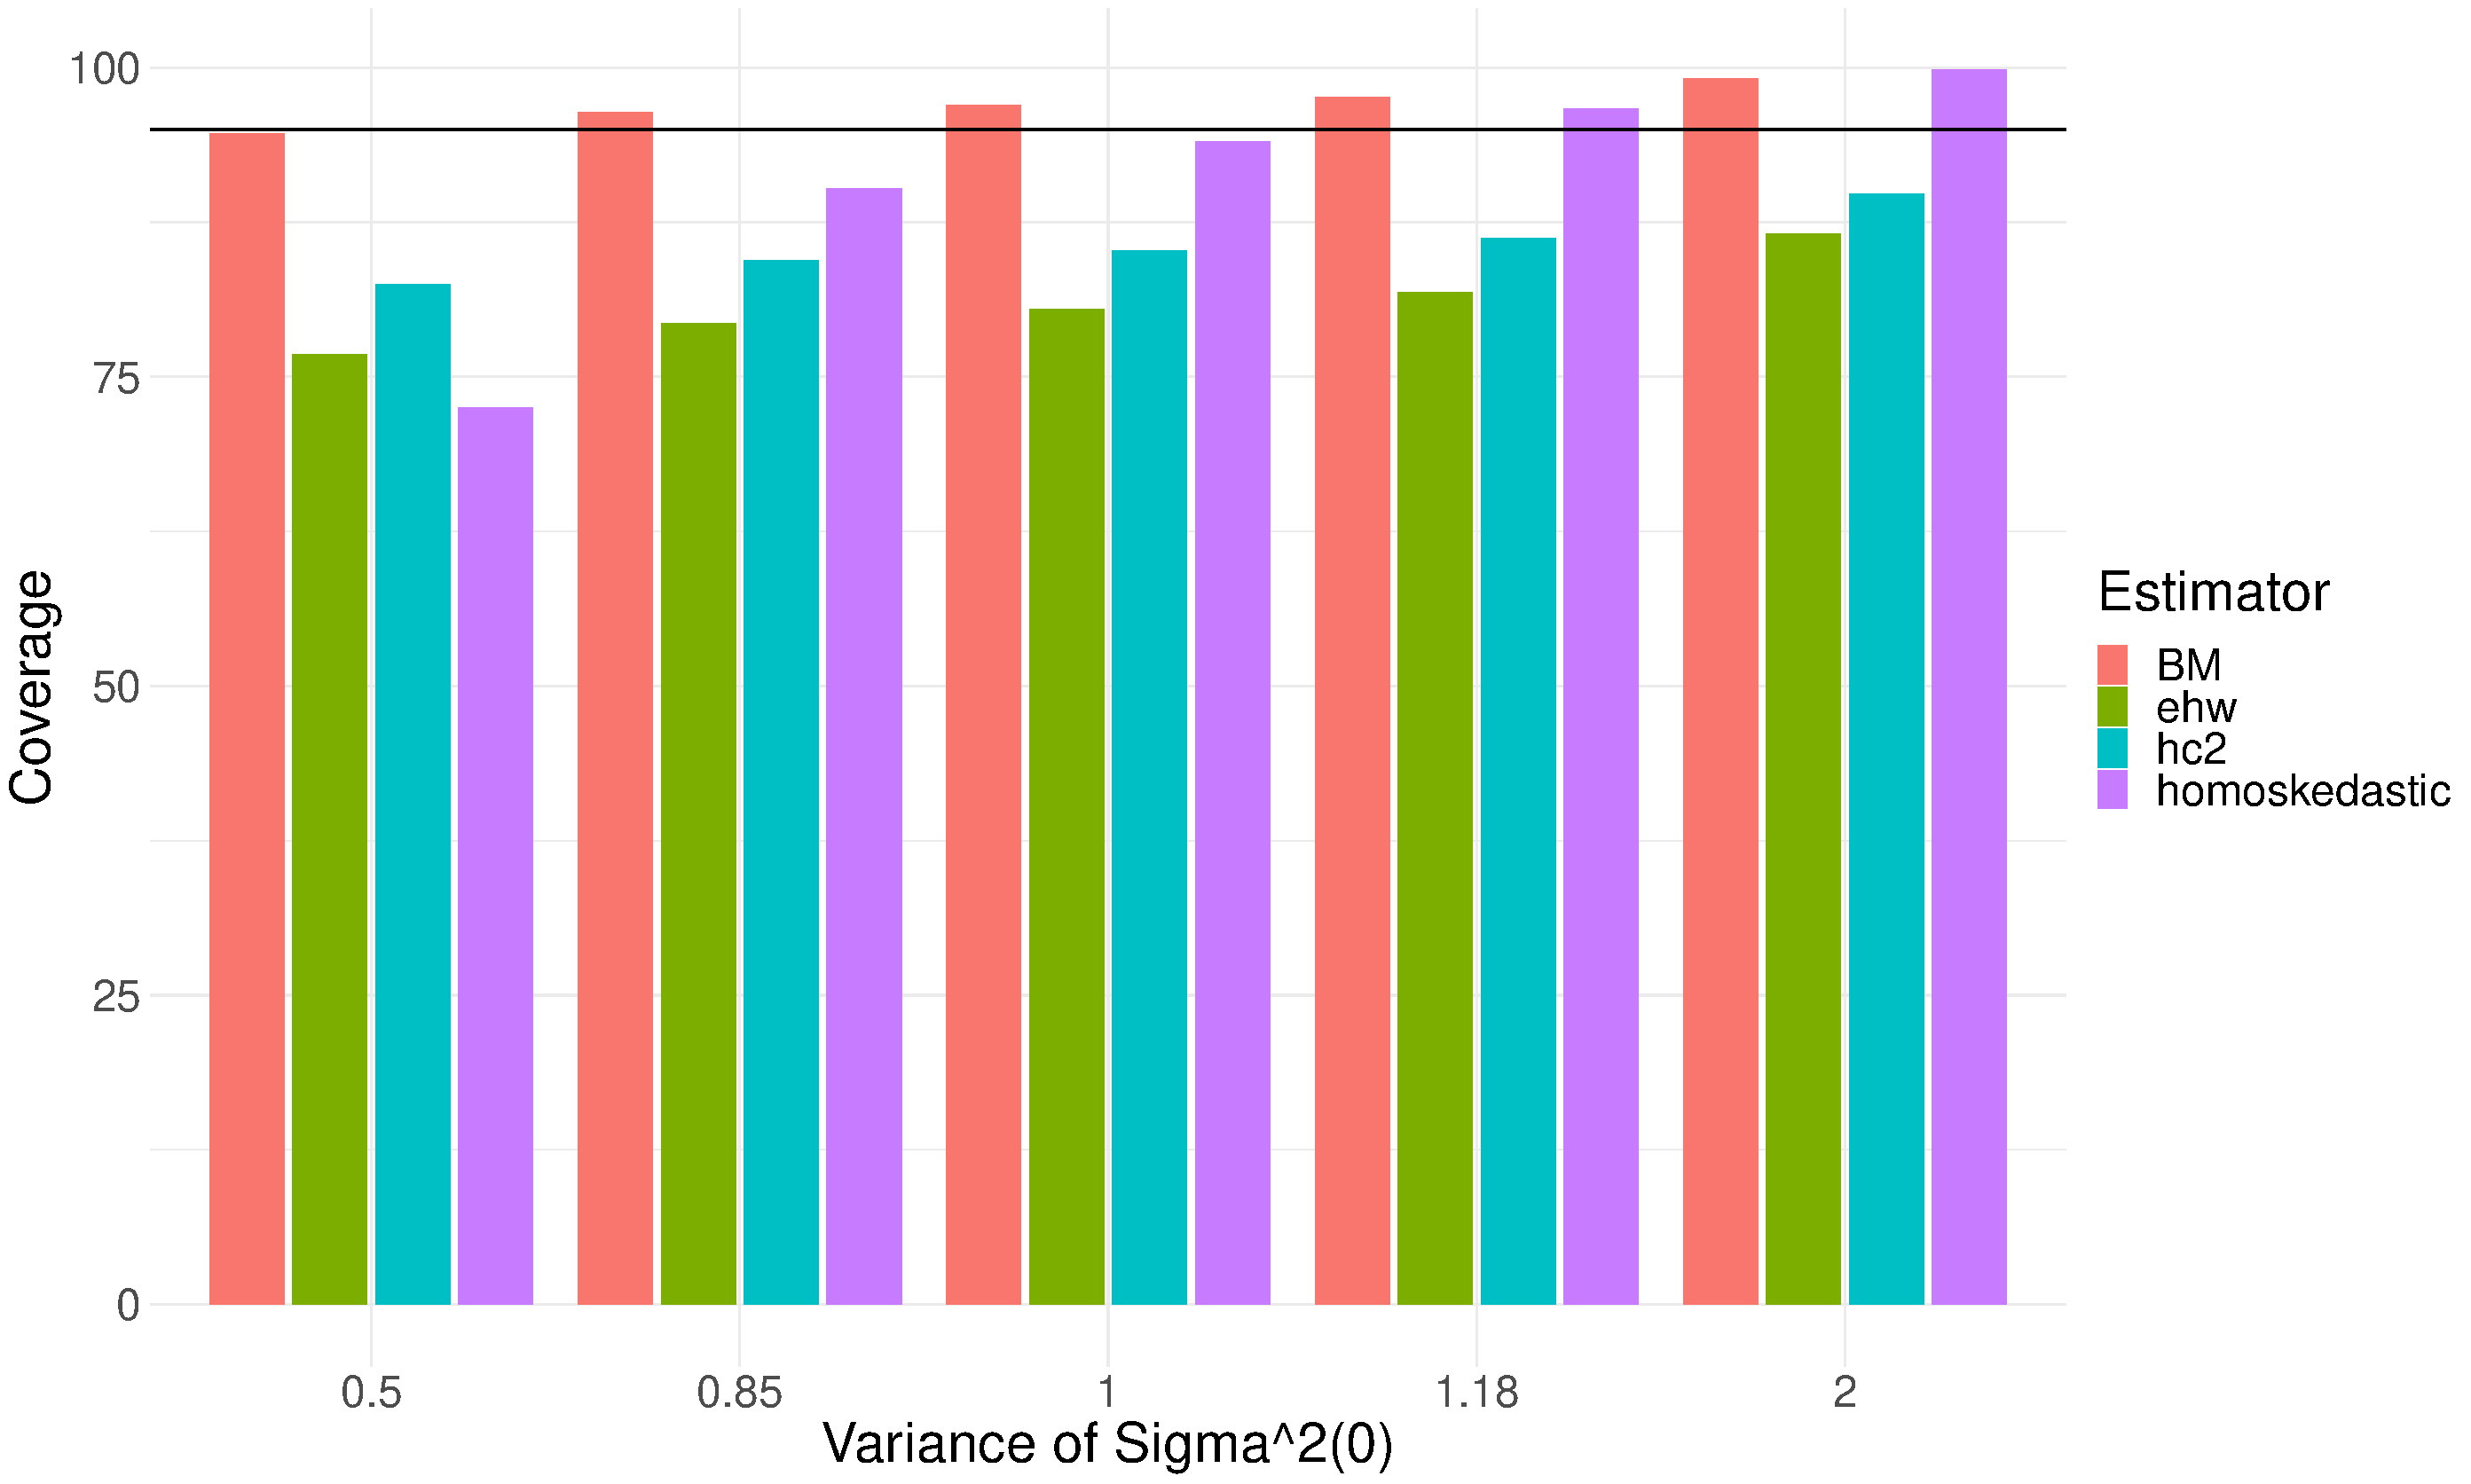
\includegraphics[width=0.7\linewidth]{images/imbenskolesar_coverage.pdf}
  \end{center}
\end{frame}


\begin{frame}{Confidence intervals and the Behrens-Fisher problem}
\begin{columns}[T] % align columns
\begin{column}{.8\textwidth}
  \begin{wideitemize}
  \item This generalizes to general regression setting (even when it's not binary)
  \item The key idea -- the variance we're scaling by is not a
    Chi-squared with the full degrees of freedom. We want to match the distribution as best we can.
  \item The approximation that we use matches the degrees of freedom
    to get the first and second moment as close as possible to the ``right'' chi-squared.
  \item This accounts for issues like a highly skewed regressor
    (log-normal right hand side variable)
  \end{wideitemize}
  \end{column}%
  \hfill%
  \begin{column}{.5\textwidth}
  \end{column}
\end{columns}
\end{frame}

\begin{frame}{Doing this in practice}
  \begin{wideitemize}
  \item These are solveable and packages exist. Stata uses the EHW 
    standard errors by default. For the Bell-Maccaffrey adjustments,
    see \texttt{reg\_sandwich}. For R, see \texttt{estimatR},
    \texttt{clubSandwich}, and Kolesar's github repo:
    \texttt{https://github.com/kolesarm/Robust-Small-Sample-Standard-Errors}
  \item Key point is that these are all approximations in finite sample
  \item What are the options for estimating $\hat{\sigma}^{2}(x)$?  
    \begin{align*}
      u_{j} &= Y_{j} - W_{j}\beta, h = \mathbf{W}(\mathbf{W}'\mathbf{W})^{-1}\mathbf{W}' & \\
          \hat{\mathbb{V}}(\hat{\beta})_{robust} &= (\mathbf{W}'\mathbf{W})^{-1}\sum_{j}(n/n-k) u_{j}^{2}W_{i}'W_{i}(\mathbf{W}'\mathbf{W})^{-1} \qquad \qquad&  \text{(robust)}\\
       \hat{\mathbb{V}}(\hat{\beta})_{HC2} &= (\mathbf{W}'\mathbf{W})^{-1}\sum_{j} (1/(1-h_{jj}))u_{j}^{2}W_{i}'W_{i}(\mathbf{W}'\mathbf{W})^{-1} \qquad \qquad& \text{(HC2)}\\
       \hat{\mathbb{V}}(\hat{\beta})_{HC3} &= (\mathbf{W}'\mathbf{W})^{-1}\sum_{j} (1/(1-h_{jj})^{2})u_{j}^{2}W_{i}'W_{i}(\mathbf{W}'\mathbf{W})^{-1} \qquad \qquad& \text{(HC3)}\\
    \end{align*}
    
  \end{wideitemize}
\end{frame}

\begin{frame}{Uncertainty -- what is it?}
  \begin{wideitemize}
  \item How should we be thinking about inference anyway? What's the error in $\epsilon$ mean anyway?
  \item The thought experiment typically comes from a sampling
    perspective -- we consider that this is a small sample from a
    broader population, and uncertainty comes from whether the estimates reflect the true underlying population
    \begin{itemize}
    \item Note that this contrasts with our design-based thought experiment!
    \end{itemize}
  \item This starts to get very confusing when thinking about some settings.
    \begin{itemize}
    \item E.g., How do we think about sampling ``new states'' when we have all 50 states?
    \item What if we have access to all the census data?
    \end{itemize}
  \item We still think we have uncertainty here when we do
    estimates. That's because there's uncertainty driven by the
    fundamental problem of causal inference!
  \end{wideitemize}
\end{frame}


\begin{frame}{Combining Sampling and Design Based uncertainty (Abadie et al. (2020))}
  \begin{wideitemize}
  \item Consider now two sources of uncertainty. There exists a population of size $N$ and a sample of size $n \leq N$.
  \item $R_{i} = \{0,1\}$ denotes whether or not an observation is in the sample
  \item There is also potential outcomes $Y^{*}(D_{i})$, driven by the
    causal variable.
  \item Now we have both sampling uncertainty (e.g. does our sample
    reflect the population) and design uncertainty (e.g. does the
    causal comparison reflect the true causal effect)
  \item But what is amazing is that we can combine the two --
    e.g. design uncertainty within a sample, versus within the
    population (internal validity vs. external validity)
  \end{wideitemize}
\end{frame}

\begin{frame}{Combining Sampling and Design Based uncertainty}
  \begin{wideitemize}
  \item   Will focus on just binary case, but paper considers full regression setting
  \item   Three estimands (apologies in advance, my $n,N$ are reversed from the paper):
  \begin{enumerate}
  \item $\theta^{descr} = N^{-1}_{1}\sum_{i=1}^{N}D_{i}Y_{i} - N^{-1}_{0}\sum_{i=1}^{N}(1-D_{i})Y_{i}$
  \item $\theta^{causal, sample} = n^{-1}\sum_{i=1}^{N}R_{i}(Y^{*}_{i}(1) - Y_{i}^{*}(0))$
  \item $\theta^{causal} = N^{-1}\sum_{i=1}^{N}(Y^{*}_{i}(1) - Y_{i}^{*}(0))$    
  \end{enumerate}
\item We have a single estimator we can consider:
  \begin{equation*}
    \hat{\theta} = n^{-1}_{1}\sum_{i=1}^{N}R_{i}D_{i}Y_{i} - n^{-1}_{0}\sum_{i=1}^{N}R_{i}(1-D_{i})Y_{i}
  \end{equation*}
\item Key point of paper -- the variance of this estimator depends on:
  \begin{enumerate}
  \item We condition on $D$ -- e.g. focus on sampling uncertainty
  \item We condition on $R$ -- e.g. focus on causal uncertainty within sample
  \item We allow for both variances
  \end{enumerate}
  \end{wideitemize}
\end{frame}

\begin{frame}{Combining Sampling and Design Based uncertainty}
  \begin{wideitemize}
  \item  What are these variances?
  \begin{enumerate}
  \item Sampling: $E(Var(\hat{\theta} | \mathbf{D}, n_{1}, n_{0}) | n_{1}, n_{0}) = \frac{S^{2}_{1}}{n_{1}}\left(1- \frac{n_{1}}{N_{1}}\right) + \frac{S^{2}_{0}}{n_{0}}\left(1- \frac{n_{0}}{N_{0}}\right),$
  \item Design:  $E(Var(\hat{\theta} | \mathbf{R}, n_{1}, n_{0}) | n_{1}, n_{0}) = \frac{S^{2}_{1}}{n_{1}} + \frac{S^{2}_{0}}{n_{0}} - \frac{S^{2}_{\theta}}{n_{1}+n_{0}}    $
  \item Both: $Var(\hat{\theta} | n_{1}, n_{0}) = \frac{S^{2}_{1}}{n_{1}} + \frac{S^{2}_{0}}{n_{0}} - \frac{S^{2}_{\theta}}{N_{1}+N_{0}}    $
  \end{enumerate}
  The $S^{2}_{\theta}$ term is what we usually ignore (because not feasibly estimable) 
\item Thought experiments:
  \begin{enumerate}
  \item Let $n$ get small relative to $N$.
  \item Not obvious which of Sampling and Design is bigger
  \item Ignoring finite sample features will lead us to overstate variance! 
  \end{enumerate}
  \end{wideitemize}
\end{frame}


\begin{frame}{Combining Sampling and Design Based uncertainty}
  Key takeaways from paper:
  \begin{enumerate}
  \item Design-based uncertainty can be smaller than traditional estimates, especially when the sample is large relative to the population
  \item Defining the relevant estimand is important for your variance estimates (e.g. causal estimates within sample, or causal estimates across populations)
    \begin{itemize}
    \item This is particularly true when your sample is a convenience sample
    \item Or, when the given sample makes sense -- e.g. 50 states
    \end{itemize}
  \item If you have a finite sample that is a non-trivial share of the population, you can improve your standard errors (see the paper)
  \item Don't get confused by the idea of having uncertainty in your
    estimates when using the population. This comes from design-based
    uncertainty, not sampling uncertainty
  \end{enumerate}
\end{frame}

\begin{frame}{Clustering and generalizing $\Omega$}
  \begin{wideitemize}
  \item   This ignored any sort of unusual correlation structure in $\Omega$, and assumed random assignment.
  \item   In many cases, we don't have that. Instead, $\Omega$  has a clustering structure
  \item This can get quite complex. Let's start with the simple case of known clusters
    \begin{itemize}
    \item E.g. units are people, and clusters are cities, counties or states
    \item For today, we're ignoring the very important quesiton of panel data
    \item We're going to discuss this! Just not today      
    \end{itemize}
  \item Let $C_{i}$ denote unit $i$'s cluster assignment. A very simple version of $\Omega$ is now
    \begin{displaymath}
      \Omega_{ij}  =\left \{\begin{array}{ccc}
                       \sigma^{2} &  \text{if}& i = j\\
                       \rho\sigma^{2}  & \text{if}&  C_{i} = C_{j} \; \& \; i \not= j\\
                       0 & \text{if} & C_{i} \not= C_{j} \; \& \; i \not= j
                     \end{array}\right.
                 \end{displaymath}
               \item Can also be more unstructured -- e.g. flexible
                 block diagonal with $\Omega_{ij} = \sigma_{ij}$ if
                 $C_{i} = C_{j}$.  Key issue -- asymptotics (see
                 Hansen (2007))
  \end{wideitemize}
\end{frame}

 
\begin{frame}{Start with the traditional model-based approach}
\begin{columns}[T] % align columns
\begin{column}{.8\textwidth}
  \begin{wideitemize}
  \item Let the number of clusters be $K$. In this case, the
    estimator for the variance of $\hat{\beta}$ (this comes from Liang
    and Zeger (1986)) is
    \begin{equation}
      \hat{\mathbb{V}}(\hat{\beta} |\mathbf{W}_{n}, \mathbf{C}_{n})_{LZ} = (\mathbf{W}_{n}'\mathbf{W}_{n})^{-1}\left(\sum_{k=1}^{K}\mathbf{W}_{k,n}'\hat{\boldsymbol{\epsilon}}_{k,n}\hat{\boldsymbol{\epsilon}}_{k,n}'\boldsymbol{W}_{k,n}\right) (\mathbf{W}_{n}'\mathbf{W}_{n})^{-1}
    \end{equation}

  \item Historically, clustering in this setting has focused the structure of $\Omega$. Why? Well, take the simple case from last slide. In this case,
    \begin{equation}
      \mathbb{V}(\hat{\beta}) = \mathbb{V}_{homoskedastic}\times \left( 1+ \rho_{\epsilon}\rho_{W}\frac{n}{K_{n}}\right),
    \end{equation}
    where $\rho_{\epsilon}$ and $\rho_{W}$ are the within-cluster correlations of each r.v.
    \vspace{-8pt}
  \item This makes you think that these are the main terms that
    matter, and more generally it's about getting the structure of
    $\Omega$ right.
    \begin{itemize}
  \item E.g., better to err on the conservative side    
    \end{itemize}
  \end{wideitemize}
  \end{column}%
  \hfill%
  \begin{column}{.5\textwidth}
  \end{column}
\end{columns}
\end{frame}


\begin{frame}{Clustering is about correlation between treatment and error}
\begin{columns}[T] % align columns
\begin{column}{.8\textwidth}
  \begin{wideitemize}
  \item However this intuition is \emph{not} correct.  (Abadie et
    al. (2017)) Can generate an example with tiny within-cluster
    correlation, and large clusters (with many clusters) where:
    \begin{itemize}
    \item $\hat{\mathbb{V}}(\hat{\beta})_{LZ}$ is large
    \item $\hat{\mathbb{V}}(\hat{\beta})_{EHW}$ is small
    \end{itemize}
  \item Why? It's all about the correlation between $W$ and
    $\epsilon$, and heterogeneity in our effects across clusters.
  \item In Abadie et al example:
    \begin{itemize}
    \item Pop = 10M, 100 equal sized clusters. Binary $W$ with
      \emph{equal} prob. = 0.5
    \item However, heterogeneous effects -- some clusters have
      positive effect, some have negative. Overall ATE is 0.
    \end{itemize}
  \item What does that mean intuitively? If there is heterogeneity in
    effects, it causes correlation between treatment and residual
    \begin{itemize}
  \item Why do the two standard errors vary so much? 
    \end{itemize}
  \end{wideitemize}
  \end{column}%
  \hfill%
  \begin{column}{.5\textwidth}
  \end{column}
\end{columns}
\end{frame}

\begin{frame}{Abadie et al}
  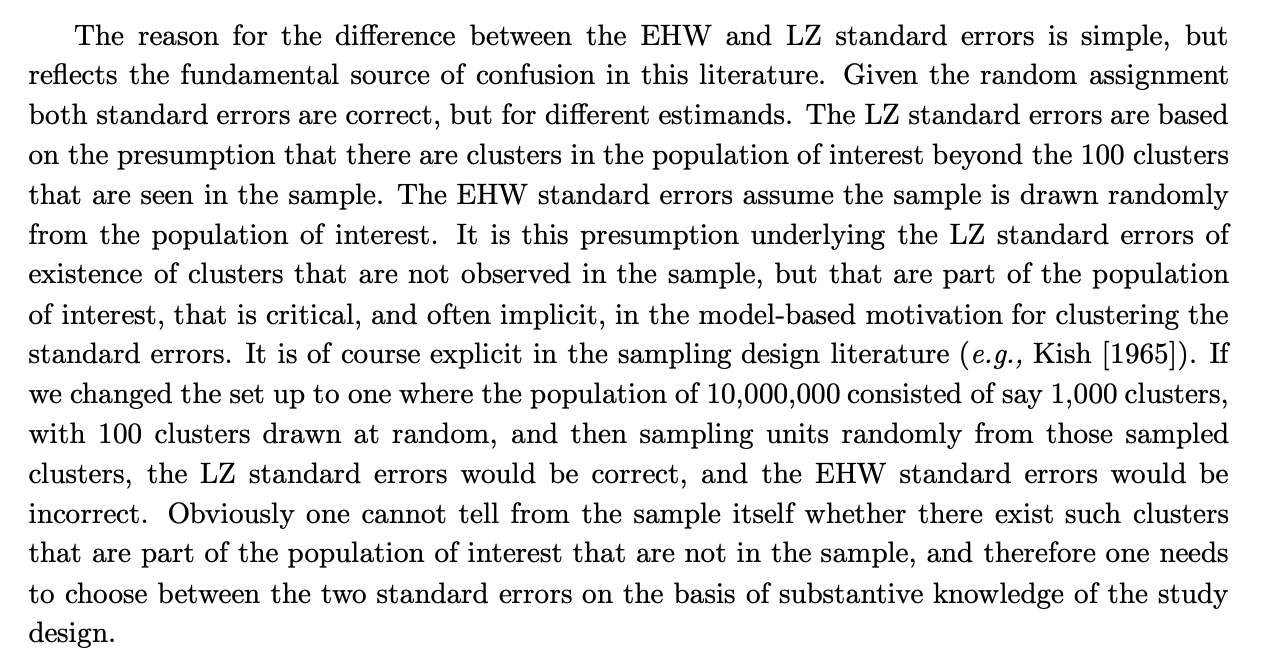
\includegraphics[width=\linewidth]{images/abadiecluster.png}
\end{frame}


\begin{frame}{Takeaways from paper}
\begin{columns}[T] % align columns
\begin{column}{.8\textwidth}
  \begin{wideitemize}
  \item Key takeaways:
    \begin{enumerate}
    \item Cluster your regression at the unit of randomization
    \item Being conservative can be quite bad! It depends on what you are trying to do.
    \item The traditional advice of being as conservative as necessary
      is likely misguided
    \item Fixed effects do NOT remove need for clstering
    \end{enumerate}
  \item We'll revisit this in panel settings. However, a question:
    what is the ``unit of randomization'' in a case like Card and
    Krueger (1993)?
    \begin{itemize}
    \item Not totally obvious. Likely impossible to say something
      truly causal without strong assumptions about simultaneous
      shocks
    \end{itemize}
  \end{wideitemize}
  \end{column}%
  \hfill%
  \begin{column}{.5\textwidth}
  \end{column}
\end{columns}
\end{frame}

\begin{frame}{Spatial and network error}
\begin{columns}[T] % align columns
\begin{column}{.8\textwidth}
  \begin{wideitemize}
  \item Things get more complicated with more general error structures.
  \item Consider two additional cases:
    \begin{itemize}
    \item Spatial correlation = $\rho_{ij} = f(d_{ij})$, where $d_{ij}$ is a function of some economic distance.
    \item Social network correlation = $\rho_{ij} = f(d_{ij})$, where $d_{ij}$ is a function of path length in a network
    \end{itemize}
  \item This can matter especially when SUTVA is violated
  \item However, Barrios et al. (2012) show that, under SUTVA, if
    treatments are randomly assigned at a given cluster level, we can
    ignore the broader spatial correlations
  \end{wideitemize}
  \end{column}%
  \hfill%
  \begin{column}{.5\textwidth}
  \end{column}
\end{columns}
  
\end{frame}

\begin{frame}{Conley (1999) distances}
\begin{columns}[T] % align columns
\begin{column}{.8\textwidth}
  \begin{wideitemize}
  \item Conley (1999) provides a flexible way to consider clustering on spatial distances.
  \item Consider our matrix $\Omega$ again. Now, $\Omega_{ij}$ is a
    function of the distance, $d_{ij}$, between each
    person. Unfortunately, this means that every person can be
    correlated.
  \item Key assumption -- the correlation declines with
    distance. Hence, far away distances matter less in
    practice. Hence, when we estimate this, we ``window'' our
    estimator (this is exactly the same as Newey-West
    estimators). Then we allow correlation as in the Liang-Zeger
    estimator, as a function of distances.
  \item This estimator is consistent for general forms of spatial
    correlation
    \begin{itemize}
    \item Estiators available in both Stata and R
    \end{itemize}
  \end{wideitemize}
  \end{column}%
  \hfill%
  \begin{column}{.5\textwidth}
  \end{column}
\end{columns}
  
\end{frame}


\begin{frame}{Consequences of ignoring spatial correlation}
\begin{columns}[T] % align columns
\begin{column}{.8\textwidth}
  \begin{wideitemize}
  \item Spatial correlation can be a big deal. Consider the analogy to time series.
    \begin{itemize}
    \item A big rule: worry about highly autocorrelated data! Can inflate your t-statistics substantially
    \item Why? Because if we treat observations as independent, we
      will infer more information than actually exists
    \end{itemize}
  \item Kelly (2019) claims that spatial correlation in outcomes can
    cause this same issue. Consider a regression of some modern
    outcome, e.g. city income, on a historical characteristic, such as
    colonial boundaries
    \begin{itemize}
    \item Claim in Kelly (2019) is that t-statistics in these types of regressions are grossly amplified by spatial correlation
    \item Fixable with Conley standard errors?
    \item This is a huge deal for a lot of literatures (economic
      history especially) -- matters for corporate governance
      literature too (LLSV)
    \end{itemize}
  \end{wideitemize}
  \end{column}
  \hfill%
  \begin{column}{.3\textwidth}
  \end{column}
  \end{columns}
\end{frame}


\begin{frame}{Final thoughts}
\begin{columns}[T] % align columns
\begin{column}{.8\textwidth}
  \begin{wideitemize}
  \item This stuff is \emph{hard}. We are doing the simplest case
    (linear regression) and still have lots of questions
  \item As always, asking what the knowable estimand is can be very helpful
  \item Next, if you are unsure, it is very useful to consider simulating data
    \begin{itemize}
    \item In many cases, there is not an obvious ``best'' answer, and simulating your data is the best solution
    \item This is because many results are asymptotic in nature, and hence approximations
    \end{itemize}
    \item Ok, so how to do simulations?
  \end{wideitemize}
  \end{column}
  \hfill%
  \begin{column}{.3\textwidth}
  \end{column}
  \end{columns}
\end{frame}


\begin{frame}{Final thoughts}
\begin{columns}[T] % align columns
\begin{column}{.8\textwidth}
  \begin{wideitemize}
  \item Goal is to generate data that matches your dataset's distributions
  \item However, for very simple simulations, you'll have to make
    parametric assumptions that may not match your actual data
  \item Athey et al. (2020) propose a method for matching the data as
    closely as possible, using a Generative Adverserial Network
  \item In other words, construct distributions that match the ``true'' data as
    closely as possible
    \begin{itemize}
    \item Computationally expensive, but great way to evaluate performance
    \item Code is available here: \url{https://github.com/gsbDBI/ds-wgan}
    \item Docs are here: \url{https://github.com/gsbDBI/ds-wgan}
    \end{itemize}
  \end{wideitemize}
  \end{column}
  \hfill%
  \begin{column}{.3\textwidth}
  \end{column}
  \end{columns}
\end{frame}



\begin{frame}{Final thoughts}
\begin{columns}[T] % align columns
\begin{column}{.5\textwidth}
  \begin{wideitemize}
  \item However this stuff is really hard to implement.
  \item If you intuitively know the issue, try doing something simple with normals
  \item Or try bootstrapping!
  \end{wideitemize}
  \end{column}
  \hfill%
  \begin{column}{.5\textwidth}
    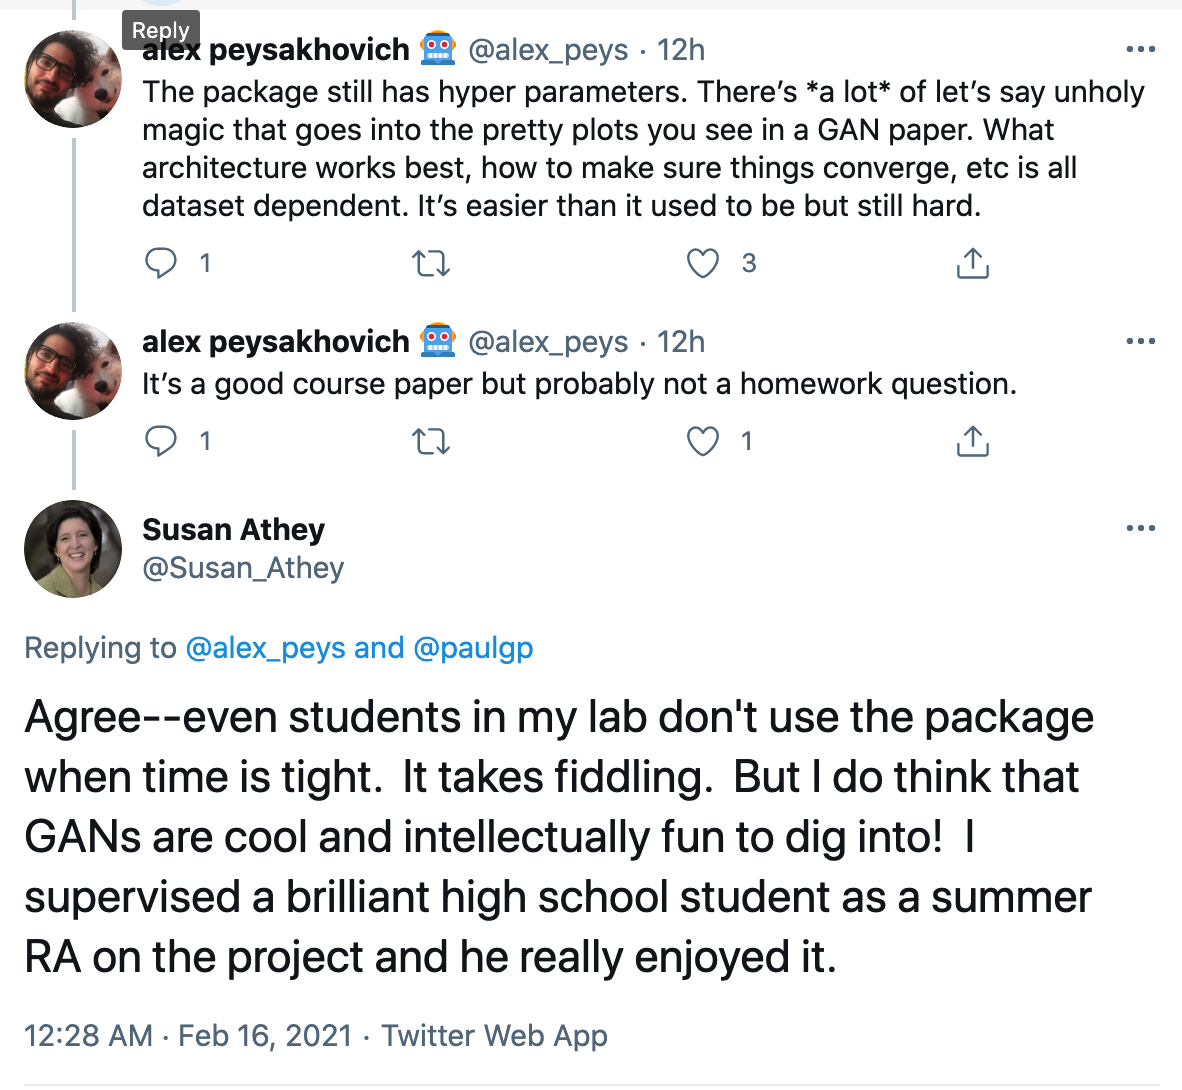
\includegraphics[width=\linewidth]{images/gan_fiddle.png}
  \end{column}
  \end{columns}
\end{frame}

\end{document}
